\documentclass[letterpaper,10pt]{article}

\usepackage{titling}
\usepackage{listings}
\usepackage{url}
\usepackage{setspace}
\usepackage{subfig}
\usepackage{sectsty}
\usepackage{pdfpages}
\usepackage{colortbl}
\usepackage{multirow}
\usepackage{multicol}
\usepackage{relsize}
\usepackage{amsmath}
\usepackage{wasysym}
\usepackage{fancyvrb}
\usepackage{amssymb}
\usepackage{ifsym}
\usepackage{amsmath,amssymb,amsthm,graphicx,xspace}
\usepackage[titlenotnumbered,noend,noline]{algorithm2e}
\usepackage[compact]{titlesec}
\usepackage{XCharter}
\usepackage[T1]{fontenc}
\usepackage{tikz}
\usetikzlibrary{arrows,automata,shapes,trees,matrix,chains,scopes,positioning,calc}
\tikzstyle{block} = [rectangle, draw, fill=blue!20, 
    text width=2.5em, text centered, rounded corners, minimum height=2em]
\tikzstyle{bw} = [rectangle, draw, fill=blue!20, 
    text width=4em, text centered, rounded corners, minimum height=2em]

\definecolor{namerow}{cmyk}{.40,.40,.40,.40}
\definecolor{namecol}{cmyk}{.40,.40,.40,.40}

\let\LaTeXtitle\title
\renewcommand{\title}[1]{\LaTeXtitle{\textsf{#1}}}


\newcommand{\handout}[5]{
  \noindent
  \begin{center}
  \framebox{
    \vbox{
      \hbox to 5.78in { {\bf ECE356: Database Systems } \hfill #2 }
      \vspace{4mm}
      \hbox to 5.78in { {\Large \hfill #4  \hfill} }
      \vspace{2mm}
      \hbox to 5.78in { {\em #3 \hfill} }
    }
  }
  \end{center}
  \vspace*{4mm}
}

\newcommand{\lecture}[3]{\handout{#1}{#2}{#3}{Lecture #1}}
\newcommand{\tuple}[1]{\ensuremath{\left\langle #1 \right\rangle}\xspace}

\addtolength{\oddsidemargin}{-1.000in}
\addtolength{\evensidemargin}{-0.500in}
\addtolength{\textwidth}{2.0in}
\addtolength{\topmargin}{-1.000in}
\addtolength{\textheight}{1.75in}
\addtolength{\parskip}{\baselineskip}
\setlength{\parindent}{0in}
\renewcommand{\baselinestretch}{1.5}
\newcommand{\term}{Winter 2018}

\singlespace


\begin{document}

\lecture{ 6 --- Data Definition }{\term}{Jeff Zarnett}

We have thus far not yet learned about how to formally create relations. It is now time to fix that. The SQL data definition language (DDL) looks a lot like the query language that we have used thus far, but it allows us to define the structure of the data. 

Specifically, our data definition language allows us to define~\cite{dsc}:
\begin{itemize}
	\item The schema of each relation.
	\item The type of each attribute.
	\item Integrity constraints.
	\item Indices on relations.
	\item Security/authorization information for a relation.
	\item Physical storage structure.
\end{itemize}

Attributes have types, and the SQL standard includes the following built in types~\cite{dsc, fds}:

\begin{itemize}
\item \textbf{char}$(n)$: A fixed length character string with a user-specified length of $n$. This one should never be used because it pads strings and it means comparisons are a pain and comparing a char attribute with another kind of string is an issue.
\item \textbf{varchar}$(n)$: A variable length character string with user-specified length $n$.
\item \textbf{int} (or \textbf{integer}): an integer (exact size and maximum value is system dependent).
\item \textbf{smallint}: a smaller integer. A fun-sized integer, so to speak.
\item \textbf{numeric}$(p, d)$: a fixed-point number with user-specified prevision; $p$ is the the number of digits and $d$ of those are to the right of the decimal point.
\item \textbf{real}: floating point with a machine-dependent precision.
\item \textbf{double precision}: double-precision floating point with machine-dependent precision.
\item \textbf{float}$(n)$: a floating point number with precision of at least $n$.
\item \textbf{boolean}: A boolean value (what did you expect?)
\item \textbf{date}, \textbf{time}, \textbf{datetime}: self explanatory, right?
\end{itemize}


\subsection*{Schema Definition - Create Table} 
If we wish to define a SQL relation, the syntax for this is to create a relation (table) is called (unsurprisingly), \texttt{CREATE TABLE}. The syntax for this command requires a name as well as a listing of the attributes (fields) and their types (definitions). It is also customary to include at least one constraint, the primary key. As before we put a semicolon at the end of the statement to designate the end of the statement. 

{\small
\begin{verbatim}
CREATE TABLE r
 (A1 D1, A2 D2, ... An Dn,
 integrity-constraint-1,
 ...
  integrity-constraint-k);
\end{verbatim}
}

A more concrete example: 
{\small
\begin{verbatim}
CREATE TABLE student
 (id varchar(8),
  userid varchar(8) NOT NULL,
  firstname varchar(64),
  lastname varchar(64),
  birthday date,
  department_id int default 0,
  PRIMARY KEY( id )
  FOREIGN KEY( department_id ) REFERENCES department( id )
 );
\end{verbatim}
}


On some attributes an additional qualifier \texttt{not null} was added, and this means that a value of \texttt{null} is forbidden from being assigned to that attribute. This is, in a way, a form of integrity constraint. Like all integrity constraints, it means an insert or update statement that tries to set such an attribute to an impermissible value will be rejected. 

The department ID attribute has a default value; if an insert statement does not specify the value for that attribute, rather than leaving it null, it will be the default value (here, 0) instead. A common case where not null and a default value could be combined is a boolean value, where the field may not be null and is by default ``false''.

The primary-key definition in this case specifies that \texttt{id} is the primary key for the relation which imposes requirements that the attribute cannot be null and must also be unique. In this situation we have defined the primary key as exactly one attribute, but a relation's primary key may be formed by the combination of several attributes. 
 
The last sort of constraint that is shown in the example is the foreign key constraint that mentions the department ID. It means that for each student, the department id value must either be null or the value must match to the id value of a department tuple. If the types of the attributes don't match (e.g., department is defined with varchar for its id rather than integer) then adding this foreign key constraint will fail. 


It is not shown in the diagram but we can override the default behaviour for what happens if the foreign key constraint is violated. Rather than rejecting the update we could choose if we want (1) to cascade the changes (alter the content of another table to make sure the rules are followed), or (2) setting null if the value is invalid, or (3) setting some default value. My personal preference is that we stick with rejection: it is better to prevent insertion of wrong data (and fix it at the source) rather than let it proceed and cover it up by putting a null in there. In the words of my friend Tuomo Jorri, if the date calculation is consistently off by 42 days, instead of a statement that says (date = date - 42), you should figure out why the date is off by 42 and fix that.

Not shown in the example above is the unique constraint: this requires simply that no two tuples of the relation may be equal in a particular attribute. Because null is not equal to null in the SQL standard, many tuples may have null for this value.

It is possible (although rare, at least in my experience) to also add a \textit{check} clause as a constraint. The check clause takes a predicate and any insertion or update is is evaluated to see if it is consistent with this constraint. A check that says \textit{salary > 0} ensures that an employee cannot be put into the database with a negative salary amount, for example~\cite{dsc}. A check constraint predicate can be arbitrarily restrictive, allowing business logic to be embedded in the database (although it is unclear if this is desirable or not).

We did not do this in the above case, but we can put a name to foreign keys or other constraints. The name must be unique in the database schema. We'll look at adding names when we talk about altering tables. Names can be useful though, because a well-named constraint can tell you what has gone wrong: if its name tells you what relations are being referenced (e.g., the key indicates it links students with departments) then if the constraint is violated on an insert or update then you know immediately what rule was being broken.

Another way that adding a foreign key might fail is if the target relation does not exist. This means we would have to create relations in some order that means the foreign keys are all satisfied at the time of the creation. That might not be realistic, though, based on the desired schema. Fortunately, we can add them in later.

\subsection*{Altering tables}

In addition to adding in some integrity constraints we can change the table definition, or remove constraints. The command for this is \texttt{ALTER TABLE} and we will need to specify the table to be modified as well as the change that we would like to make. 

If we want to add a new column to the table, then the alter table syntax requires us to specify the name of the new attribute to be added and the type. \texttt{ALTER TABLE students ADD COLUMN email VARCHAR(128);} Subsequent to that we can make additional changes, such as adding an index, or putting in a reference constraint (which we will see how to do soon). At the time of creation, we can set a default value or set an attribute to be not null, however. Note that is is possible to add multiple elements in a single statement. 

The mirror operation to that is to drop a column: \texttt{ALTER TABLE students DROP COLUMN email;} This deletes the attribute from the database and all the data that is in there, permanently. Dropping the column can fail if the column is used in a foreign key or other constraint. It may also be necessary to remove an index... 

If we wish to rename a table, the keyword we need is \texttt{RENAME}: \texttt{ALTER TABLE students RENAME users;} This would change the name of the students relation to be \texttt{users}. It is not very exciting.

To change the definition of a column, we can use \texttt{MODIFY} or \texttt{CHANGE} depending on what we want to do: \texttt{ALTER TABLE users MODIFY email VARCHAR(255);} changes the definition of the email attribute; if we use \texttt{CHANGE} we have to specify the new definition including the name.

To add an index to a table, we (may) need a name for the index, and specify the relation and attribute(s) it should be created on: \texttt{CREATE INDEX idx\_lastname ON users (lastname);}. But we don't have to, we could use a slightly different syntax: \texttt{ALTER TABLE users ADD INDEX (lastname);} which creates an index without needing to give it a name. In truth, it will be given a default name, but you at least don't need to make one up. Management of an index is not specified in the SQL standard so there's a fair amount of difference between the various vendors.

To remove an index, \texttt{ALTER TABLE users DROP INDEX lastname;}. If we didn't explicitly give the index a name it is likely the name of the column itself. If we really have no idea what the name of an index is, we can use \texttt{SHOW INDEX FROM users;} to ask the server to give us the information we need.

To add a foreign key, it gets complex: we need to define both tables first. Suppose there is a login session for an application and it is associated with a user's id attribute. To add a constraint we need to:

\begin{verbatim}
ALTER TABLE sessions
ADD CONSTRAINT FK_SESSION_USER
FOREIGN KEY (userid) REFERENCES users(id);
\end{verbatim}

There is alternative syntax along the lines of \texttt{ADD FOREIGN KEY} but as a design decision I discourage it. In the above example the foreign key gets a name \texttt{FK\_SESSION\_USER} which is helpful in debugging. Adding the foreign key constraint in this way will fail if the two attributes (userid and id) do not have the same domain (e.g., they are not both varchar with length 8). Worse than that, if one of the tables is defined in one character encoding (UTF-8) and the other is defined in a different encoding (UTF-8mb4) then adding the constraint will fail and it might seem like a mystery as to why!

To remove a foreign key: \texttt{ALTER TABLE users DROP FOREIGN KEY FK\_SESSION\_USER;}


\subsection*{Truncate Table}

If we wish to remove all tuples from a relation without affecting the structure at all, the command for that is to truncate the table: \texttt{TRUNCATE TABLE students;} would remove from the database all tuples of the students relation but would leave its definition unchanged. Truncating the table may fail if it would violate some constraints (breaking referential integrity).

There are some scenarios where this is a desirable operation. One possible scenario is if you have some application where login session information is stored in the database and you want to invalidate and remove all sessions you can truncate the table.

\subsection*{Drop Table}

If we wish to remove a relation from the schema, the syntax for this is \texttt{DROP TABLE students}. This deletes the table and all of its content and then the content is permanently lost. And again, the drop operation may fail if the table to be deleted is referenced in some external constraints.

\begin{center}
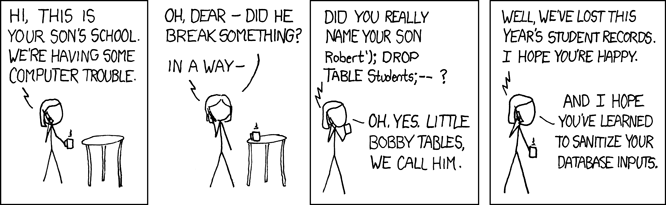
\includegraphics[width=0.7\textwidth]{images/exploits_of_a_mom}\\
Obligatory XKCD ( \url{https://xkcd.com/327/} ).
\end{center}

\subsection*{Stored Procedures}
It is possible to define our own procedures in database server and save them and embed them into the database. Rather than having application logic stored solely in the application program we can embed some of it in the database. It can also enforce some separation of the logic: rather than the application program manipulate tables directly, the application calls the stored procedures and the procedures manipulate the database tables.

It is possible to write procedures in SQL (which is what we'll do in this course) but there may be support for writing it in another programming language (e.g., C or Java). One objective of this course is to be proficient in SQL so delegating everything to another programming language is undesirable. More than that, though, it is important to use procedures judiciously: simple SQL statements or even complex ones may be sufficient to get the job done; if everything is done in procedures then we miss out on the opportunity to learn to think about accomplishing the goal in the correct way. 

It is worth noting that we can also define functions, which are similar to procedures but not identical. To reduce confusion and keep it simple we will focus just on procedures. 

When we want to create a procedure, we need to give it a name, define the parameters and make a statement about whether the procedure is deterministic. Then there is the body of the procedure.

You will notice that nothing was said about return value. That's because a procedure does not have one: parameters are defined as \texttt{IN}, \texttt{OUT}, or \texttt{INOUT}. In parameters are the default and it means of course that it is an input parameter and changes are not made to the original input; out means it is a returned value so its initial value in the procedure is null until assigned; inout means it is taken as input and (possibly) modified before being returned.

On the subject of whether the procedure is deterministic, the mysql manual\footnote{\url{https://dev.mysql.com/doc/refman/5.7/en/create-procedure.html}} says the following:

\begin{quote}
A routine is considered ``deterministic'' if it always produces the same result for the same input parameters, and ``not deterministic'' otherwise. If neither \texttt{DETERMINISTIC} nor \texttt{NOT DETERMINISTIC} is given in the routine definition, the default is \texttt{NOT DETERMINISTIC}. To declare that a function is deterministic, you must specify \texttt{DETERMINISTIC} explicitly.

Assessment of the nature of a routine is based on the ``honesty'' of the creator: MySQL does not check that a routine declared \texttt{DETERMINISTIC} is free of statements that produce nondeterministic results. However, misdeclaring a routine might affect results or affect performance. Declaring a nondeterministic routine as \texttt{DETERMINISTIC} might lead to unexpected results by causing the optimizer to make incorrect execution plan choices. Declaring a deterministic routine as \texttt{NONDETERMINISTIC} might diminish performance by causing available optimizations not to be used.
\end{quote}

Enough introduction: let's look at a very simple example from~\cite{dsc}:

{\small
\begin{verbatim}
CREATE PROCEDURE dept_count_proc( IN dept_name VARCHAR(20), OUT d_count INTEGER )
BEGIN
  SELECT COUNT(*) INTO d_count
  FROM instructor
  WHERE instructor.dept_name = dept_count_proc.dept_name
END
\end{verbatim}
}

To create a procedure, the keywords are unsurprisingly \texttt{CREATE PROCEDURE}, followed by the name of the procedure. We observe that there is one in parameter and one out parameter. The order does not have to be in parameters before out parameters. The body of the function is bracketed with the \texttt{BEGIN} and \texttt{END} statements that are like the opening and closing braces on a function in a C-like language.

In a practical sense we probably want to have multiple statements and when we are giving in the create procedure statement we do not want a semicolon to result in detecting the end of the statement too early. The common solution to this is to bracket the create procedure statement with statements that change the delimiter (end of statement code). The syntax is \texttt{DELIMITER //} which then changes, from that point on, the delimiter to be \texttt{//}. Then at the end, we change it back to a semicolon with \texttt{DELIMITER ;}. The double slash delimiter is just convention, it could be anything, and some texts use \texttt{\$\$} instead.

{\small
\begin{verbatim}
DELIMTER //
CREATE PROCEDURE proc () 
DETERMINISTIC
BEGIN
  DECLARE a INT;
  SET a = 42;
  INSERT INTO table1 ( a );
END//
DELIMITER ;
\end{verbatim}
}

The procedure above shows the use of the delimiter changing syntax as well as putting DETERMINISTIC and a multi line procedure, and some new things we haven't seen before such as declaring variables and assigning them. To provide a quick summary of the syntax from~\cite{storedproc} we can do the following things: declare variables, assign them, and use flow control structures like if-statements, and we can iterate with a cursor.

Declaration of a variable is pretty simple, you simply declare the variable using \texttt{DECLARE} with a name and data type (and an optional default value) such as the statement above. To assign it, use \texttt{SET} as above. 

To understand how if-statements work, we'll do a comparison against a typical C like language:

\begin{multicols}{2}
\begin{lstlisting}[language=C]
if ( x == 0 ) {
  y = 1;
} 
\end{lstlisting}
\columnbreak
\begin{verbatim}
IF x = 0 THEN
  SET y = 1;
END IF;
\end{verbatim}
\end{multicols}

Aside from the fact that the if condition is no longer in brackets and the equality is tested with a single equals sign, the big difference is the presence of the \texttt{THEN} as well as \texttt{END IF} keywords, in place of the usual curly braces. We can extend that with an else block as well:

\begin{multicols}{2}
\begin{lstlisting}[language=C]
if ( x == 0 ) {
  y = 1;
} else {
  y = 2;
}
\end{lstlisting}
\columnbreak
\begin{verbatim}
IF x = 0 THEN
  SET y = 1;
ELSE
  SET y = 2;
END IF;
\end{verbatim}
\end{multicols}

There are of course loops (and there's a goto statement, but please don't...). We'll cover the while-loop, but it's not the only kind there could be; there are also other keywords...

\begin{multicols}{2}
\begin{lstlisting}[language=C]
while ( y > 0 ) {
  y = y - 1;
} 
\end{lstlisting}
\columnbreak
\begin{verbatim}
WHILE y > 0 DO
  SET y = y - 1;
END WHILE;
\end{verbatim}
\end{multicols}

If you want to iterate over rows returned by a query and perform some action on them, then the command for that is \texttt{CURSOR}. Use of a cursor is complex and there are several parts we need to do.

{\small
\begin{verbatim}
DECLARE e VARCHAR(128);
DECLARE quit BOOLEAN;

DECLARE cursor1 CURSOR FOR 
  SELECT email FROM USERS;
DECLARE CONTINUE HANDLER FOR NOT FOUND
  SET quit = TRUE;  
OPEN cursor1;

loopname: LOOP
  IF quit = TRUE THEN
    LEAVE loopname;
  END IF;

  FETCH cursor1 INTO e;
  # do something useful with e

END LOOP loopname;
CLOSE c1;
\end{verbatim}
}

Creation of a cursor is done with the \texttt{DECLARE} statement as shown; it takes the result of a select statement. That is the set that we will iterate over. Then we need to indicate our ending condition, what to do when we get to the end of the data set. The usual correct answer for that is to break out of the loop and go on to the next step, as is done here. Then the \texttt{OPEN} command actually carries out the select statement and loads the data for the cursor to iterate over. Then we have our loop; we use the \texttt{FETCH} command to load the next variable into e; after which we can do something useful with it (not shown here for space reasons). It's worth noting that the loop has a name (loopname) which we use to break out of the loop if the quit condition is fulfilled. After the loop there is a close statement which frees up the memory allocated for the cursor.

Cursors don't update their data set if the underlying table is changed in the meantime; that's why the open statement exists and why its placement can matter. Open it at the last minute to get the most up to date data. Cursors are read only, and they always advance from one item to the next and never go backwards or skip anything.

By default, the procedure you create has autocommit set to ``on'' so any changes made are performed immediately, even if you have a multi line statement. That is not necessarily what you want; it may be that you want the whole block of statements to be processed as a single transaction (yes!). If that is the case then some additional syntax should be added. At the beginning of the transaction, add \texttt{START TRANSACTION;}. If everything goes well and you are ready for your changes to be saved, use the statement \texttt{COMMIT;}. If for some reason you need to cancel your changes and don't want them to be saved, then use \texttt{ROLLBACK;} instead of the commit statement. As fun as it might be to go through a detailed example, that might give away a little too much for one of the labs...

To trash a procedure, the syntax is just \texttt{DROP PROCEDURE dept\_count\_proc;}. There does exist a limited ability to alter a procedure, but don't do it; if you need to change a procedure, it is best to drop and re-create it.

Finally, to call a stored procedure, the keyword is \texttt{CALL} followed by the procedure name, and, obviously, the arguments the procedure needs in parenthesis. If there are no arguments needed, empty parenthesis are used.

\subsection*{Triggers}

It is possible to define an operation in the database that will take place automatically when some other modification of the database takes place. As you might imagine from the name, it follows a logic of ``if $x$ happens, then do $y$''. 

To define a trigger we need to define~\cite{dsc}:
\begin{itemize}
	\item An event that causes the trigger to be checked.
	\item A condition that must be satisfied for actions to be taken.
	\item The actions to be taken.
\end{itemize}

Triggers are useful in a few scenarios. They can be used to cause some events to occur such as updating related data, checking an integrity constraint that would be too difficult to check any other way, or alerting humans that some condition is satisfied. I generally discourage the first use: application logic should probably be the one that modifies the data. Checking integrity is a good use. Alerting humans is usually something like sending an email... No program is complete unless it sends e-mail.

Let's do an example from~\cite{trigger} where there is a ``blog'' table with blog posts (sure, why not) and an audit table that stores deleted entries so they can be recovered if we want.

{\small
\begin{verbatim}
DELIMITER $$
CREATE TRIGGER blog_after_insert 
  AFTER INSERT 
  ON blog
  FOR EACH ROW 
  BEGIN
  
  IF NEW.deleted THEN
    SET @changetype = 'DELETE';
  ELSE
    SET @changetype = 'NEW';
  END IF;  
  INSERT INTO audit (blog_id, changetype) VALUES (NEW.id, @changetype);
		
  END$$
DELIMITER ;
\end{verbatim}
}

There are further options, of course, and this is only a specific example. The \texttt{AFTER INSERT} statement tells us the time (either before or after) and the event is one of \texttt{INSERT}, \texttt{UPDATE}, or \texttt{DELETE}. If there are multiple triggers on the same condition we can specify an order on them by name, saying that it \texttt{PRECEDES} or \texttt{FOLLOWS} some other trigger. And then we have the trigger body which starts with the for-each row and begin statements. The operations of the body are done on each row that satisfies the conditions of the trigger

In the body, the row being inserted is pointed to by the \texttt{NEW} keyword. In an update there is also the \texttt{OLD} keyword to reference the old row. A delete has only the \texttt{OLD} row and there is no \texttt{NEW}.

The example does not have a \texttt{WHEN} condition, but it is possible to have one which allows to specify a condition that limits when this trigger performs the action (without an if block where one branch is blank). 


\bibliographystyle{alphaurl}
\bibliography{356}


\end{document}
